\documentclass[12pt]{article}

% ------------------------------
% PAQUETES BÁSICOS
% ------------------------------
\usepackage[utf8]{inputenc}
\usepackage[T1]{fontenc}
\usepackage[spanish, es-nodecimaldot]{babel} % <- punto decimal
\decimalpoint
\usepackage{amsmath, amssymb, amsfonts}
\usepackage{graphicx}
\usepackage{geometry}
\usepackage{fancyhdr}
\usepackage[
    backend=biber,
    style=numeric,
    sorting=none
]{biblatex}
\addbibresource{biblio.bib}
\usepackage{caption}
\usepackage{subcaption}
\usepackage{enumitem}
\usepackage{hyperref}
\usepackage{xcolor}
\usepackage{booktabs} % tablas bonitas

% ------------------------------
% CONFIGURACIÓN GENERAL
% ------------------------------
\geometry{letterpaper, margin=2.5cm}
\setlength{\parskip}{0.5em}
\setlength{\parindent}{0pt}

% Cambiar "Cuadro" por "Tabla"
\addto\captionsspanish{\renewcommand{\tablename}{Tabla}}

% ------------------------------
% ENCABEZADO Y PIE DE PÁGINA
% ------------------------------
\pagestyle{fancy}
\fancyhf{}
\chead{\textbf{Técnicas Estadísticas y Minería de Datos}}
%\lhead{\textbf{TEyMD}}
%\rhead{\textbf{Tarea 5}}


% Pie de página con línea superior
\renewcommand{\footrulewidth}{0.4pt} % grosor de la línea (0 para quitarla)
\rfoot{\thepage}
\lfoot{\textbf{Harold Vázquez Corrilo}}
% ------------------------------
% COLORES Y LINKS
% ------------------------------
\hypersetup{
    colorlinks=true,
    linkcolor=blue!60!black,
    urlcolor=blue!60!black,
    citecolor=green!60!black
}

% ------------------------------
% INICIO DEL DOCUMENTO
% ------------------------------
\begin{document}

%\begin{center}
 %   {\LARGE \textbf{Tarea 1}}\\[4pt]
  %  {\large Curso: Nombre del curso}\\[2pt]
   % {\large Profesor: Nombre del profesor}\\[2pt]
    %{\large Fecha: \today}
%\end{center}

%\hrule
%\vspace{1em}
\newcommand{\m}[1]{\pmb{#1}} % comando para vectores y matrices en negrita


%%%%%%
%% Tema: Cointegración
%%%%%%

\subsection*{Cointegración}

\begin{itemize}
    \item \textbf{Prueba de Johansen:}\\
    La prueba de Johansen es un método que permite detectar la presencia de relaciones de cointegración entre múltiples series temporales.
    Parte del vector autorregresivo (VAR) de orden $p$ 
    \begin{align}
        \pmb{y}_t = \m{\mu} + \m{A}_1 \m{y}_{t-1} + \m{A}_2 \m{y}_{t-2} + ... + \m{A}_p \m{y}_{t-p} + \m{\varepsilon}_t,
        \label{eq:var}
    \end{align}
    donde $\pmb{y_t}$ es un vector de $M$ variables integradas de orden uno $I(1)$ que se creen cointegradas,
    $\pmb{\mu}$ es un vector de constantes, $\m{A}_i$ son matrices de coeficientes y 
    $\pmb{\varepsilon_t}$ es un vector de errores blancos. La expresión \eqref{eq:var} se puede reescribir 
    en forma de corrección de errores (VEC) como:
    \begin{align}
        \Delta \pmb{y}_t = \pmb{\mu} + \m{\Pi} \m{y}_{t-1}+ \sum_{i=1}^{p-1} \m{\Gamma}_i \Delta \pmb{y}_{t-i} + \pmb{\varepsilon}_t,
    \end{align}
    donde $\Delta$ es el operador de diferencia, $\m{\Pi} = -\pmb{I} + \sum_{i=1}^{p} \pmb{A}_i$ y
    $\m{\Gamma}_i = -\sum_{j=i+1}^{p} \pmb{A}_j$. La matriz $\m{\Pi}$ contiene información sobre las relaciones de cointegración, ya que
    si el rango de $\m{\Pi}$ es $r$ (donde $r < M$), entonces existen las matrices  de tamaño $(M \times r)$ $\m{\alpha}$ y $\m{\beta}$ 
    tales que $\m{\Pi} = \m{\alpha} \m{\beta}'$ y $\m{\beta}' \m{y}_t$ es estacionaria. Aquí, $\m{\beta}$ contiene los vectores de cointegración y $\m{\alpha}$ 
    contiene los coeficientes de ajuste en el modelo de corrección de errores \cite{Osterholm2007Testing}.\\
    Johansen propone dos estadísticas de prueba: la estadística de traza y la estadística de valor máximo propio. Las expresiones son:
    \begin{align}
        \text{Estadístico de traza: } & \quad J_{\text{traza}} = -T \sum_{i=r+1}^{M} \ln(1 - \hat{\lambda}_i) \\
        \text{Estadístico de valor máximo propio: } & \quad J_{\text{max}} = -T \ln(1 - \hat{\lambda}_{r+1}),
    \end{align}
    donde $T$ es el número de observaciones, $\hat{\lambda}_i$ es el $i$-ésimo mayor valor de correlación canónica estimado entre $\Delta \pmb{y}_t$ y $\pmb{y}_{t-1}$.\\
    La estadística de traza prueba la hipótesis nula de $r$ vectores de cointegración contra 
    la hipótesis alternativa de $M$ vectores de cointegración, mientras que la estadística de valor máximo propio prueba la hipótesis nula de $r$ vectores de cointegración
    contra la hipótesis alternativa de $r+1$ vectores de cointegración \cite{Osterholm2007Testing}.

    \item \textbf{Interpretación del coeficiente del MCE:}\\
    Considerando dos series de tiempo $I(1)$ $Y_t$ y $X_t$ y que se tiene el modelo de corrección de errores (MCE):
    \begin{align}
        \Delta Y_t = \alpha_0 + \alpha_1 \Delta X_t + \alpha_2 \text{mce}_{t-1} + \varepsilon_t,
        \label{eq:mce}
    \end{align}
    donde $\text{mce}_{t-1} = Y_{t-1} - \beta_0 - \beta_1 X_{t-1}$ es el término de corrección de errores. En este 
    modelo, el valor absoluto de $\alpha_2$ indica la velocidad con la que se restablece el equilibrio entre las dos series 
    después de una desviación \cite{gujarati_econometri_2015} y se le conoce como el coeficiente de ajuste.
    
    \item \textbf{Aplicaciones de la cointegración:}\\
    La cointegración y los modelos de corrección de errores se han utilizado para crear modelos macroeconómicos
    donde se han utilizado casi todas las variables macroeconómicas principales, como inversión, impuestos,
    consumo, empleo, tasas de interés, gasto público, etc. Los cuales son de utilidad para bancos centrales, el 
    Federal Reserve Bank y otras instituciones para simulaciones de políticas económicas \cite{granger2004}.\\
    Otra aplicación es la de resolver muchas de las dificultades que aparecen cuando a dos series 
    integradas se les aplica una regresión y parece haber una relación, cuando en realidad no la hay.
    Es decir, que la cointegración ayuda a resolver los problemas relacionados con regresiones espurias \cite{granger2004}.
    Esto provocó que muchos editores tuvieran que revisar de nuevo artículos que ya habían sido aceptados.\\
    
\end{itemize}

%%%%%%%%%%%%%%%%%%%
%%%%%%%% Tema : Diagnóstico 
%%%%%%%%%%%%%%%%%%%

\subsection*{Diagnóstico del modelo con MCE}
Se realizó el diagnóstico del modelo con MCE de la data 3-6 (ver figura \ref{fig:mce_modelo}), las pruebas realizadas y los resultados obtenidos se muestran a continuación.
\begin{figure}[h!]
    \begin{center}

        Modelo 2: MCO, usando las observaciones 1960--1994 ($T$ = 35)\\
        Variable dependiente: pc\_Ct\\
        
        \vspace{1em}
        
        \begin{tabular}{lr@{.}lr@{.}lr@{.}lr@{.}l}
          &
         \multicolumn{2}{c}{Coeficiente} &
          \multicolumn{2}{c}{Desv.\ Típica} &
           \multicolumn{2}{c}{Estadístico $t$} &
            \multicolumn{2}{c}{valor p} \\[1ex]
        const &
          0&406198 &
            0&271409 &
              1&497 &
                0&1443 \\
        pc\_Yt &
          0&839422 &
            0&0939651 &
              8&933 &
                0&0000 \\
        mce\_1 &
          $-$0&00179869 &
            0&000977668 &
              $-$1&840 &
                0&0751 \\
        \end{tabular}
        
        \vspace{1ex}
        \begin{tabular}{lrlr}
        Media de la vble. dep. &  2.265466 & D.T. de la vble. dep. &  1.878602 \\
        Suma de cuad. residuos &  34.22190 & D.T. de la regresión &  1.034135 \\
        $R^2$ &  0.714796 & $R^2$ corregido &  0.696971 \\
        $F(2, 32)$ &  40.10019 & Valor p (de $F$) &  1.92\textrm{e--09} \\
        Log-verosimilitud & $-$49.26941 & Criterio de Akaike &  104.5388 \\
        Criterio de Schwarz &  109.2049 & Hannan--Quinn &  106.1495 \\
        $\hat{\rho}$ &  0.017734 & Durbin--Watson &  1.926095 \\
        \end{tabular}
        \end{center}
    \caption{Modelo con MCE de la data 3-6.}
    \label{fig:mce_modelo}     
\end{figure}

\begin{itemize}
    \item \textbf{Pruebas de normalidad y media cero:}\\
    Se realizaron distintas pruebas para determinar si los residuos del modelo con MCE siguen una distribución normal.\\
    \begin{table}[h!]
    \centering
    \begin{tabular}{lc}
        \toprule
        Prueba & Valor p \\
        \midrule
        Doornik-Hansen & 0.144324 \\
        Shapiro-Wilk & 0.0788871 \\
        Lilliefors & 0.03 \\
        Jarque-Bera & 0.326355 \\
        Chi-cuadrado & 0.14432 \\
        \bottomrule
    \end{tabular}
    \caption{Valores p de las pruebas de normalidad para los residuos del modelo con MCE.} 
    \label{tab:residuos_normalidad}
    \end{table}
    \begin{figure}[h!]
        \centering
        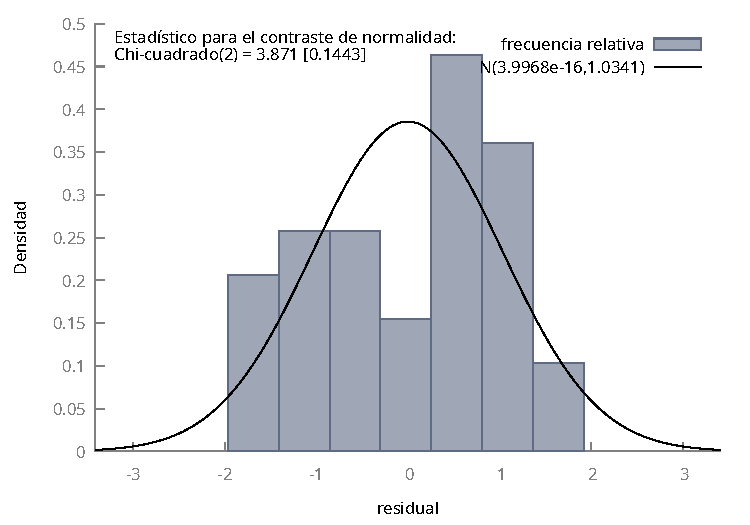
\includegraphics[width=0.55\textwidth]{imagenes/hist_res.pdf}
        \caption{Histograma de los residuos del modelo con MCE.}
        \label{fig:residuos_hist}
    \end{figure}\\
    Se observa en la tabla \ref{tab:residuos_normalidad} que la mayoría de las pruebas no 
    rechazan la hipótesis nula de normalidad al 5\% de significancia, excepto la prueba de Lilliefors.
    Dado que la mayoría de las pruebas no rechazan la hipótesis nula, se puede considerar que los residuos 
    siguen una distribución normal.\\
    Además, en la figura \ref{fig:residuos_hist} podemos observar que la media de los residuos es
    $\mu = 3.9968 \times 10^{-16}$ que es un valor muy cercano a cero, por lo que se puede considerar que los residuos
    tienen media cero.

    \item \textbf{Pruebas de heterocedasticidad:}\\
    Para el caso de la heterocedasticidad, primero se observó el comportamiento de los residuos
    a través del tiempo (ver figura \ref{fig:residuos_time}).\\
    \begin{figure}[h!]
        \centering
        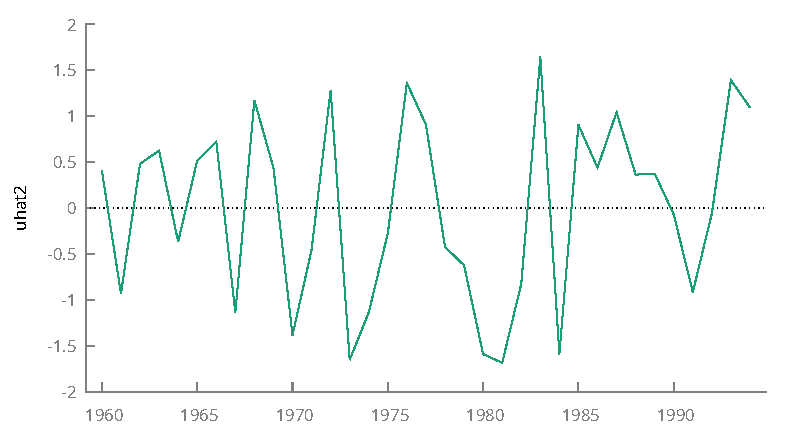
\includegraphics[width=0.55\textwidth]{imagenes/resi_graf.pdf}
        \caption{Residuos del modelo con MCE a través del tiempo.}
        \label{fig:residuos_time}
    \end{figure}\\
    A simple vista, no se observa que la amplitud de los residuos se expanda o contraiga sistemáticamente
    a lo largo del tiempo. Sin embargo, para confirmar esta observación, se realizó la prueba de 
    heterocedasticidad de White, donde se obtuvo un valor $$p = 0.040780 $$ y la prueba de heterocedasticidad
    de White (solo cuadrados), donde se obtuvo un valor $$p= 0.0972637$$.\\
    Sabemos que la prueba de White puede servir como prueba de heterocedasticidad o de error de especificación,
    por lo tanto le damos más importancia a la prueba de White (solo cuadrados) para evaluar la heterocedasticidad,
    ya que esta es una prueba más específica para este propósito. Dado que el valor p de esta prueba es mayor
    al nivel de significancia del 5\%, no se rechaza la hipótesis nula de homocedasticidad. Por lo tanto, concluimos 
    que los residuos del modelo con MCE son homocedásticos.

    \item \textbf{Pruebas de autocorrelación:}\\
    Se realizó la prueba LM de autocorrelación con diferentes retardos para evaluar la presencia de autocorrelación en los residuos,
    los resultados se muestran en la tabla \ref{tab:LM_autocorr}.
    \begin{table}[h!]
    \centering
    \begin{tabular}{lc}
        \toprule
        Retardos & Valor p \\
        \midrule
        1 & 0.891812 \\
        10 & 0.919783 \\
        15 & 0.641928 \\
        \bottomrule
    \end{tabular}
    \caption{Valores p de la prueba LM de autocorrelación.}
    \label{tab:LM_autocorr}
    \end{table}\\
    Además de la prueba LM, el estadístico Durbin-Watson se calculó y se obtuvo un valor de 1.92609, con
    los siguientes valores p:
    \begin{itemize}
        \item $H_1$: autocorrelación positiva $p=0.340253$
        \item $H_1$: autocorrelación negativa $p=0.659747$
    \end{itemize}
    Observando los valores p en la tabla \ref{tab:LM_autocorr} y los del estadístico Durbin-Watson, concluimos 
    que la evidencia estadística indica que no hay autocorrelación en los residuos del modelo con MCE.

    \item \textbf{Prueba de multicolinealidad:}\\
    Se realizó la prueba de multicolinealidad calculando el factor de inflación de la varianza (VIF) para las variables explicativas,
    obteniéndose los siguientes resultados:
    \begin{itemize}
        \item VIF de $pc\_Yt$: 1.019
        \item VIF de $\text{mce}\_1$: 1.019
    \end{itemize}
    Sabemos que un valor de VIF menor a 10 indica que el grado de multicolinealidad es bajo. Dado que ambos valores de VIF son cercanos a 1,
    concluimos que no hay multicolinealidad entre las variables explicativas del modelo.


    \item \textbf{Pruebas de cambios estructurales:}\\
    La primera prueba que se realizó fue RV de Quandt, obteniendo un valor $$p_{\text{asintótico}} = 0.410786$$ y 
    el siguiente gráfico:
    \begin{figure}[h!]
        \centering
        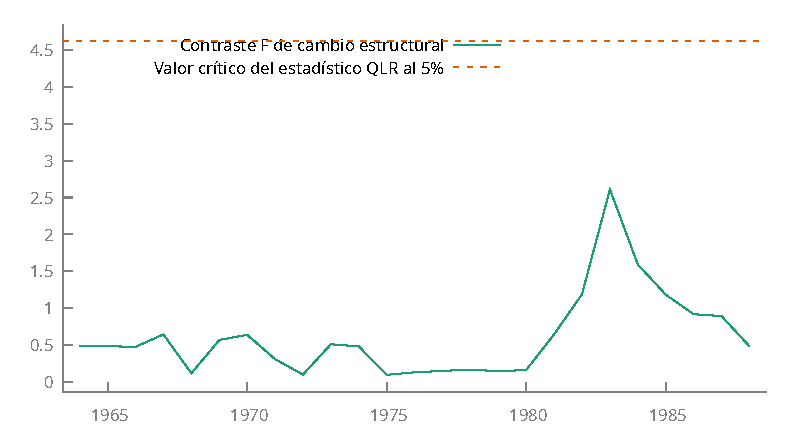
\includegraphics[width=0.55\textwidth]{imagenes/rv_quandt.pdf}
        \caption{Gráfico de la prueba RV de Quandt.}
        \label{fig:rv_quandt}
    \end{figure}\\
    Notamos que durante todos los años el valor del estadístico esta por debajo de la linea
    punteada roja, esta observación y el valor $p$ nos da indicios de que puede que no existan 
    cambios estructurales.\\
    Además, se realizaron las pruebas CUSUM y CUSUMSQ, obteniéndose los siguientes gráficos:
    \begin{figure}[h!]
        \centering
        \begin{subfigure}[b]{0.47\textwidth}
            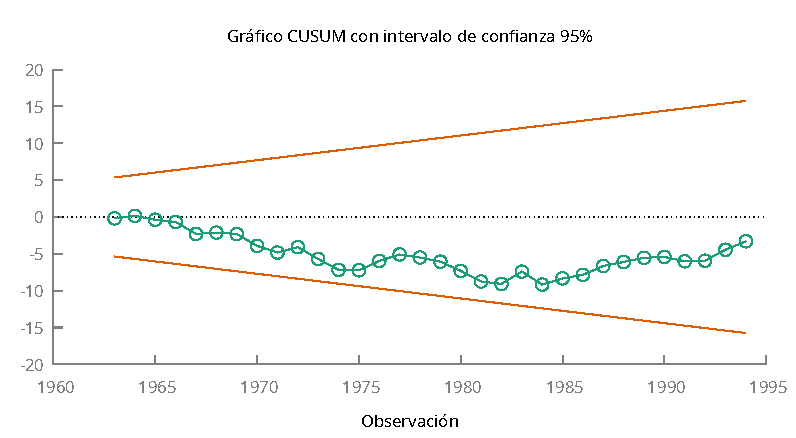
\includegraphics[width=0.9\textwidth]{imagenes/cusum.pdf}
            \caption{Prueba CUSUM.}
            \label{fig:cusum}
        \end{subfigure}
        \hfill
        \begin{subfigure}[b]{0.47\textwidth}
            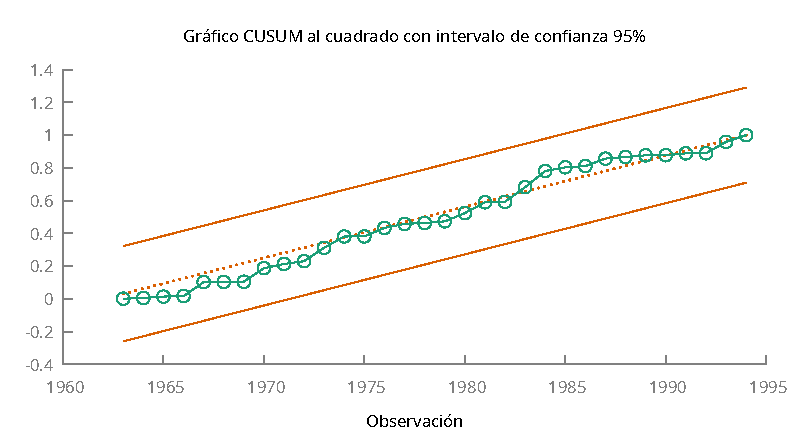
\includegraphics[width=0.9\textwidth]{imagenes/cusumsq.pdf}
            \caption{Prueba CUSUMSQ.}
            \label{fig:cusumsq}
        \end{subfigure}
        \caption{Gráficos de las pruebas CUSUM y CUSUMSQ.}
        \label{fig:cusum_cusumsq}
    \end{figure}\\
    Notamos que estas pruebas tampoco muestran evidencia de cambios estructurales, ya que en ambos gráficos 
    los puntos se mantienen dentro de las líneas de confianza. Por lo tanto, concluimos 
    que no hay cambios estructurales.
    
    \item \textbf{Pruebas de forma funcional lineal:}\\
    Se realizaron las pruebas RESET de Ramsey de solo cuadrados y solo cubos, obteniéndose los siguientes valores p:
    \begin{itemize}
        \item RESET (solo cuadrados): $p = 0.00922474$
        \item RESET (solo cubos): $p = 0.00546949$
    \end{itemize}
    Notamos que ambas pruebas rechazan la hipótesis nula de especificación adecuada.\\
    También se realizó la prueba de no linealidad (cuadrados) y se obtuvo un valor $$p = 0.00839665.$$ 
    En este caso se rechaza la hipótesis nula de linealidad.\\
    En conclusión, las pruebas de forma funcional lineal indican que el modelo tiene errores de forma funcional
    y con base en la prueba de no linealidad, podría pensarse en incluir términos cuadrados de las variables explicativas.


    \item \textbf{Pruebas de adición u omisión de variables:}\\
    Debido a que la data solo contiene dos variables, no se pudieron realizar pruebas de adición u omisión de variables.

\end{itemize}







\printbibliography

% ------------------------------
% FIN DEL DOCUMENTO
% ------------------------------
\end{document}